\chapter{Results}

Our results include game input taxonomies, a user-defined game input set, user ratings, subjective responses, and qualitative observations for each interaction method.

  \begin{table}
    \centering
    \begin{tabular}{|l|l|l|l|l|}
      \hline
      \tabhead{Method} &
      \multicolumn{1}{|p{0.13\columnwidth}|}{\centering\tabhead{Mean}} &
      \multicolumn{1}{|p{0.13\columnwidth}|}{\centering\tabhead{Std.}} &
      \multicolumn{1}{|p{0.13\columnwidth}|}{\centering\tabhead{L.Bound}} &
      \multicolumn{1}{|p{0.13\columnwidth}|}{\centering\tabhead{U.Bound}} \\
      \hline
      handheld & 3.68 & 0.79 & 3.63 & 3.74\\
      \hline
      touch & 3.77 & 0.81 & 3.72 & 3.83\\
      \hline
      non-touch & 3.81 & 0.90 & 3.75 & 3.87\\
      \hline

    

    \end{tabular}
    \caption{Summary of user preference of 3 different interaction methods, it provides mean value, standard deviation, and 95\% confidence interval for mean (Lower Bound and Upper Bound).}
    \label{tab:tablePreferenceInteractionMethod}
  \end{table}

  \section{Preference Between Interaction Methods}
  Table \ref{tab:tablePreferenceInteractionMethod} shows the average rating of 3 interaction methods. Three interaction types had a significant rating difference ($F_{0.05}$(2, 2445)=4.61, $p$ = .01). We found that the user rating preference for \emph{non-touch} was significantly higher than for \emph{handheld} ($p$ = .009). And we didn't find a significant difference between \emph{touch} and \emph{non-touch} ($p$ = .688).
  
  In the interview conducted after the rating, we asked why users gave \emph{handheld} a lower preference score.
  The general reason was that users had to take their controller, e.g. phone, out of their pocket first. Users thought the handheld controller was not always-available and was not hands-free compared to the other interaction methods in this study. After analysing the video recording, we found that most participants simply used the handheld device as a trackpad. In addition, the user behavior and mental model were similar to the previous work by Liang et al.\cite{Liang:2012:USG:2350046.2350098}. Considering the users' preferences and the reasons mentioned above, our report will focus on the results of \emph{touch} and \emph{non-touch} interaction.

  \section{Behavior with Different Form Factor of Glasses}
  In our study, for each of the two glasses, there are 1224 game input pairs with the user, task and interaction method. We found 119 pairs of game input (9.72\% of all) were designed differently with distinct smart glasses forms. The influence of game input in each interaction method was 1.22\% for \emph{handheld}, 7.35\% for \emph{touch} and 20.59\% for \emph{non-touch}.

  While using \emph{non-touch} as interaction method, users who designed distinctive game input action mentioned that they were eager to use direct control and perfom a in-air gesture in front of the screen with the Epson Moverio. However, it is difficult to perform the same input with Google Glass because of the small screen size. On the other hand, users' reasons to define different input with different glasses for \emph{touch} and \emph{handheld} interaction methods seem to be random as users were unable to motivate their choice to define a different input.

  Although the form factor of smart glasses influenced the design of game inputs, there was almost no difference in the user preference ratings for user-defined game inputs between the 2 different glasses: ($F_{0.05}$(1, 2446)=.36, $p$=.549).


  \section{Classification of Game Inputs}
  %As noted in related work, ???????? . Ho however, no work has established a taxonomy of game control based on user behavior in public space to capture and describe the game design space.

   \begin{table}
    \centering
    \begin{tabular}{|c|l|c|}
      \hline
      \tabhead{\#} &
      \multicolumn{1}{|p{0.4\columnwidth}|}{\centering\tabhead{Task}} &
      \multicolumn{1}{|p{0.2\columnwidth}|}{\centering\tabhead{Kappa Value}} \\
      \hline
      1 & Select single from many& 0.863\\
      \hline
      2 & Vertical menu & 1.000\\
      \hline
      3 & Horizontal menu & 0.688\\
      \hline
      4 & Move left and right & 0.825\\
      \hline
      5 & Move in 4 directions & 1.000\\
      \hline
      6 & Switch 2 objects & 0.804\\
      \hline
      7 & Move object to position & 1.000\\
      \hline
      8 & Draw a path & 1.000\\
      \hline
      9 & Throw an object (in-2D) & 1.000\\
      \hline
      10 & Follow the beats & 0.697\\
      \hline
      11 & Rotate an object (Z-axis) & 0.867 \\
      \hline
      12 & Rotate an object (Y-axis) & 1.000\\
      \hline
      13 & Avatar jump & 0.867\\
      \hline
      14 & Avatar 3D move & 0.880\\
      \hline
      15 & Avatar attack & 1.000\\
      \hline
      16 & Avatar squat & 0.878\\
      \hline
      17 & Control 3D viewport  & 0.878\\
      \hline
      & \bf{Average} & \bf{0.897}\\
      \hline

    \end{tabular}
    \caption{Inter-rater reliability for each task.}
    \label{tab:kappa}
  \end{table}


  \subsection{Taxonomy of Game Input}
       
  As the authors, we manually classified the input actions along four dimensions: \emph{form}, \emph{binding}, \emph{nature}, and \emph{flow}. Within each dimension, there are multiple categories as shown in Table \ref{tab:taxonomy}. To verify the objectivity (or inter-rater reliability), we invited an independent rater who performed the same categorization using 170 trials (10 trials were randomly selected for each task). The inter-rater reliability is shown in Table \ref{tab:kappa}. The lowest Kappa value, .688, is greater than .6, which is rated as \textsl{substantial} and thus is sufficient to establish the validity of the categorization. In addition, the average Kappa value is .897. A Kappa value of .8 and higher is considered \textsl{almost perfect}\cite{kappavalue}.

  \begin{table}
    \centering
    \begin{adjustwidth}{-0.5cm}{}
    \begin{tabular}{|l|l|l|}
      \hline
      \multicolumn{3}{|p{1.06\columnwidth}|}{\centering\tabhead{\textbf{Taxonomy of Game Inputs}}}\\
      \Xhline{4\arrayrulewidth}
        \textbf{\em{Form}} & \em{palm} & I.b. finger and palm. \\ \cline{2-3} 
        \textbf{\em{{\fontsize{0.3cm}{1em}\selectfont (touch)}}} & \em{fingers} & I.b. fingers.\\ \cline{2-3} 
             & \em{leg} & I.b. finger and leg.\\ \cline{2-3} 
             & \em{back of hand} & I.b. finger and back of hand.\\ \cline{2-3} 
             & \em{forearm} & I.b. finger and forearm.\\ \cline{2-3} 
             & \em{face} & I.b. finger and face.\\ \cline{2-3} 
             & \em{wrist} & I.b. finger and wrist.\\ \cline{2-3} 
             & \em{ring} & I.b. finger and ring. \\ \cline{2-3} 
             & \em{watch} & I.b. finger and watch.\\ \cline{2-3} 
             & \em{glasses} & I.b. finger and glasses.\\ \cline{2-3} 
             & \em{necklace} & I.b. finger and necklace.\\ 
       \Xhline{4\arrayrulewidth}
        \textbf{\em{Form}} & \em{finger} & Using finger to perform in-air gesture.\\ \cline{2-3} 
        \textbf{\em{{\fontsize{0.3cm}{1em}\selectfont (non-touch)}}}  & \em{hand} & Using hand to perform in-air gesture.\\ \cline{2-3} 
             & \em{head} & Using head to perform input.\\ \cline{2-3} 
             & \em{voice} & Using voice control.\\ 
      \Xhline{4\arrayrulewidth}
        \textbf{\em{Binding}} & \em{direct} & Directly control in front of screen. \\ \cline{2-3} 
             & \em{surface} & Absolute mapping screen to surface.\\ \cline{2-3} 
             & \em{independent} & No binding b. screen and input.\\
      \Xhline{4\arrayrulewidth}
        \textbf{\em{Nature}} & \em{symbolic} & Input visually depicts a symbol.\\ \cline{2-3} 
             & \em{physical} & Input acts physically on objects.\\ \cline{2-3} 
             & \em{metaphorical} & Input indicates a metaphor.\\ \cline{2-3} 
             & \em{abstract} & Input mapping is arbitrary.\\
      \Xhline{4\arrayrulewidth}
        \textbf{\em{Flow}} & \em{discrete} & Response occurs \em{after} the user acts.\\ \cline{2-3} 
             & \em{continuous} & Response occurs \em{before} the user acts.\\
      \hline
    \end{tabular}
    \caption{Taxonomy of game inputs based on 2448 input actions. The abbreviation ``I.b.'' means ``Interaction between''. The abbreviation ``b.'' means ``between''.}
    \label{tab:taxonomy}
    \end{adjustwidth}
  \end{table}
 

  

  The scope of the \emph{Form} dimension is applied separately to different interaction methods. There are 11 \emph{Form} categories with \emph{touch} input. 4 of them (\emph{palm}, \emph{back of hand}, \emph{forearm}, \emph{wrist}) are performed with both hands. 2 of them (\emph{leg}, \emph{face}) use a single hand to interact with other body parts. \emph{fingers} is a single hand input and it is merely an interaction between fingers, e.g. a pinch. And rest of them (\emph{ring}, \emph{watch}, \emph{glasses}, \emph{necklace}) are interactions with accessories. There are 4 form categories with the \emph{non-touch} interaction method. \emph{Finger} is a special case of \emph{hand}, but it is worth distinguishing because of its similarity to mouse actions and direct-touch.


  In the \emph{Nature} dimension, \emph{symbolic} inputs are visual depiction. For example, a user poses the v-sign in the air in order to select menu option 2, or forms his hand as a gun to throw an object. \emph{physical} inputs with the virtual object should be similar to the real world interaction with the physical object. \emph{metaphorical} inputs occur when an input acts on, with, or like something else. For instance, users trace a finger in a circle to simulate the ``object rotation'', or view the palm as a trackpad to perform gestures. As it should be, the input itself is usually not enough to reveal its metaphorical nature; the answer lies in the user's mental model which could be understood by the interview afterwards. Finally, \emph{abstract} inputs have no \emph{symbolic}, \emph{physical}, or \emph{metaphorical} connection to their game tasks. The mapping is arbitrary, which does not necessarily mean it is poor. Pinch-touching thumb and index finger to perform ``avatar jump'', for example, would be an abstract input.

The \emph{Binding} dimension is defined as the relationship between the input area and the smart glass's screen. \emph{direct} binding means the user performs the inputs in the screen region directly, such as using an in-air gesture right in front of the screen to drag or touch virtual objects. A game input binding is called a \emph{surface} binding if the user absolutely maps the screen onto another surface and performs the game inputs on it. Dragging a finger on the palm to move the object on the screen, for example, is a \emph{surface} binding input. For inputs categorized as \emph{independent} inputs it means that there is no binding between the screen and the input area. Thus the input can be performed in any position, like the ``pinch to jump''.

  A game input's \emph{Flow} is \emph{discrete} if the input is performed, delimited, recognized, and responded to as an event. An example is punching in the air to perform ``avatar attack''. \emph{Flow} is \emph{continuous} if ongoing recognition is required, such as during most of our participants' ``Control 3D viewport'' rotating the imaginary camera by hands. 

  

 \subsection{Taxonometric Breakdown of Input Actions in our Data}
We found that our taxonomy adequately describes even widely differing input actions made by our users. Figure \ref{fig:OnBodyTaxonomy} and \ref{fig:InAirTaxonomy} show for each dimension the percentage distribution between the categories. The \emph{Form} dimension for \emph{touch} input and the the \emph{Form} dimension for \emph{non-touch} input are both dominated with hand related input. And \emph{Form} dimension for \emph{touch} input is consisted of \emph{On-Body}(80.3\%) and \emph{Wearable}(19.7\%) interaction. We found that the forms of \emph{touch} inputs are more complicated than those of \emph{non-touch}. Nonetheless, the binding of \emph{touch} is more consistent. About 75\% of the inputs are independent of the screen. In addition, we were surprised that no user designed a \emph{direct} binding or \emph{physical} nature input with \emph{touch} input. And we found that for the \emph{Flow} dimension, the percentage distribution is similar to \emph{touch} and \emph{non-touch} interaction.

 \begin{figure}[h]
  \centering
  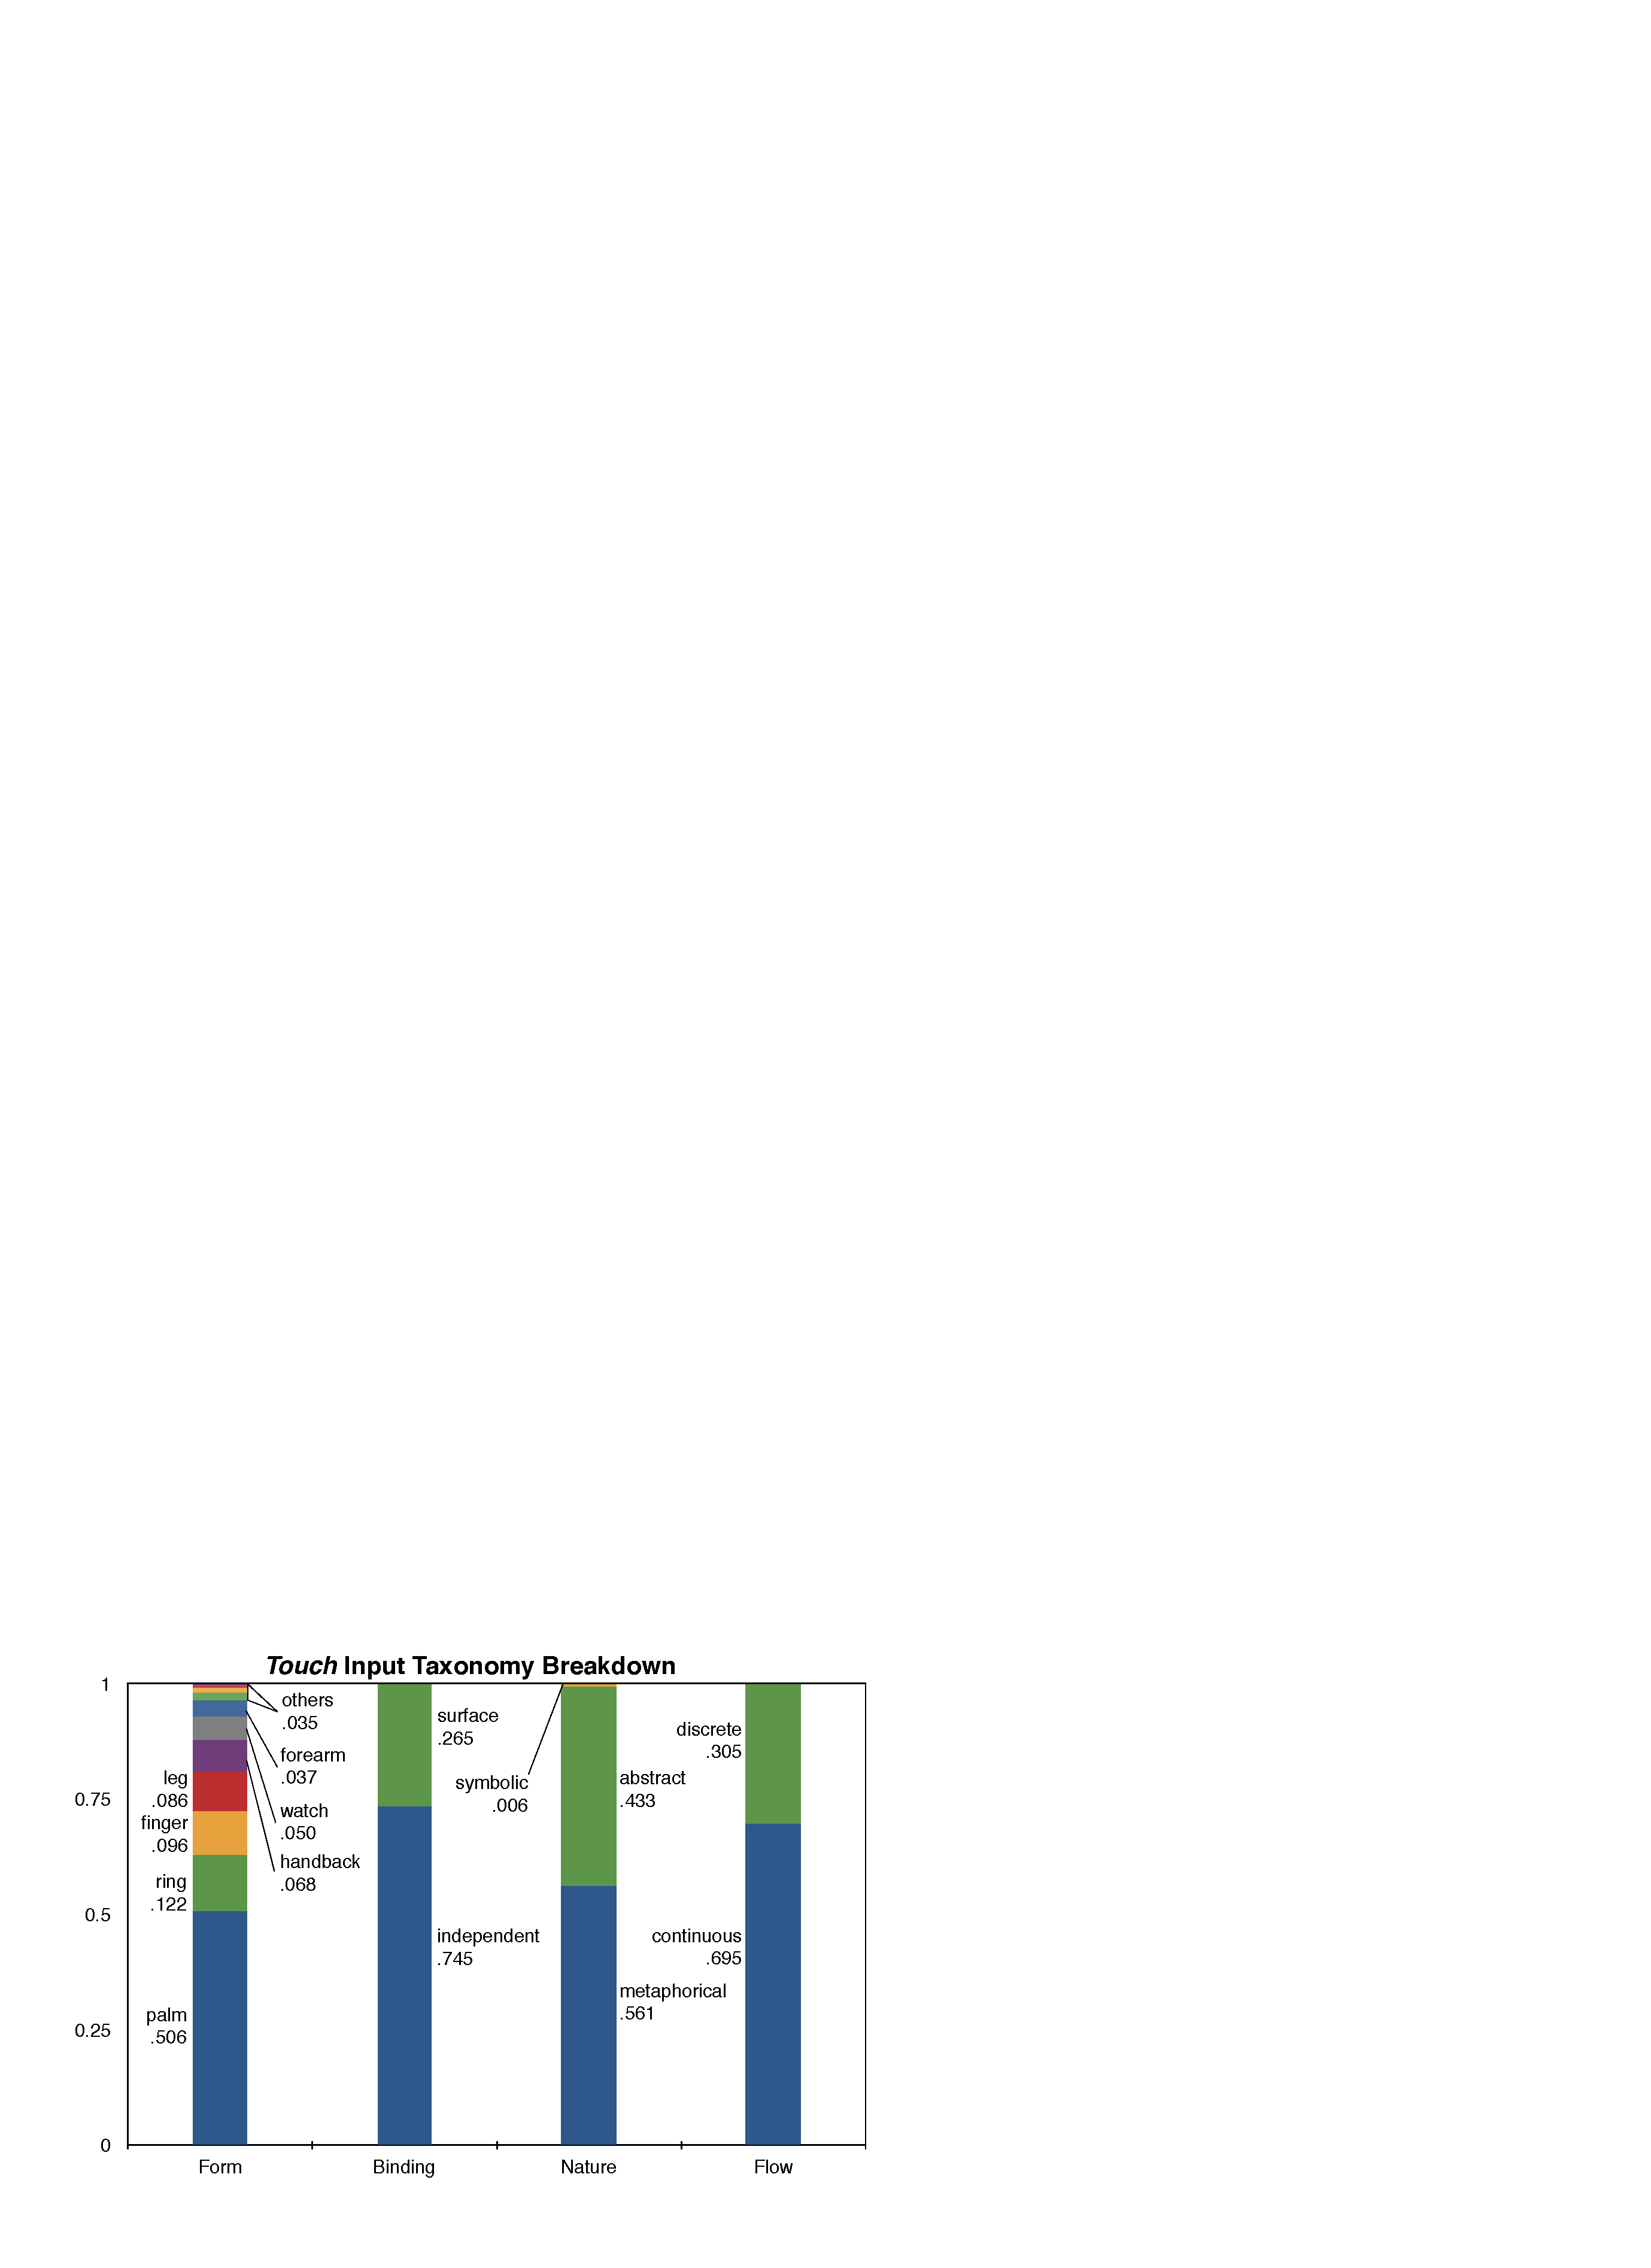
\includegraphics[width=1.0\columnwidth]{Figures/OnBodyTaxonomy}
  \caption{Percentage of game inputs in each taxonomy dimension with \emph{touch} interaction. The  ``others'' on the form dimension is consisted of glasses (0.0164), necklace (0.0088), face (0.0075) and wrist (0.0025).}
  \label{fig:OnBodyTaxonomy}
  \end{figure} 

  \begin{figure}[h]
  \centering
  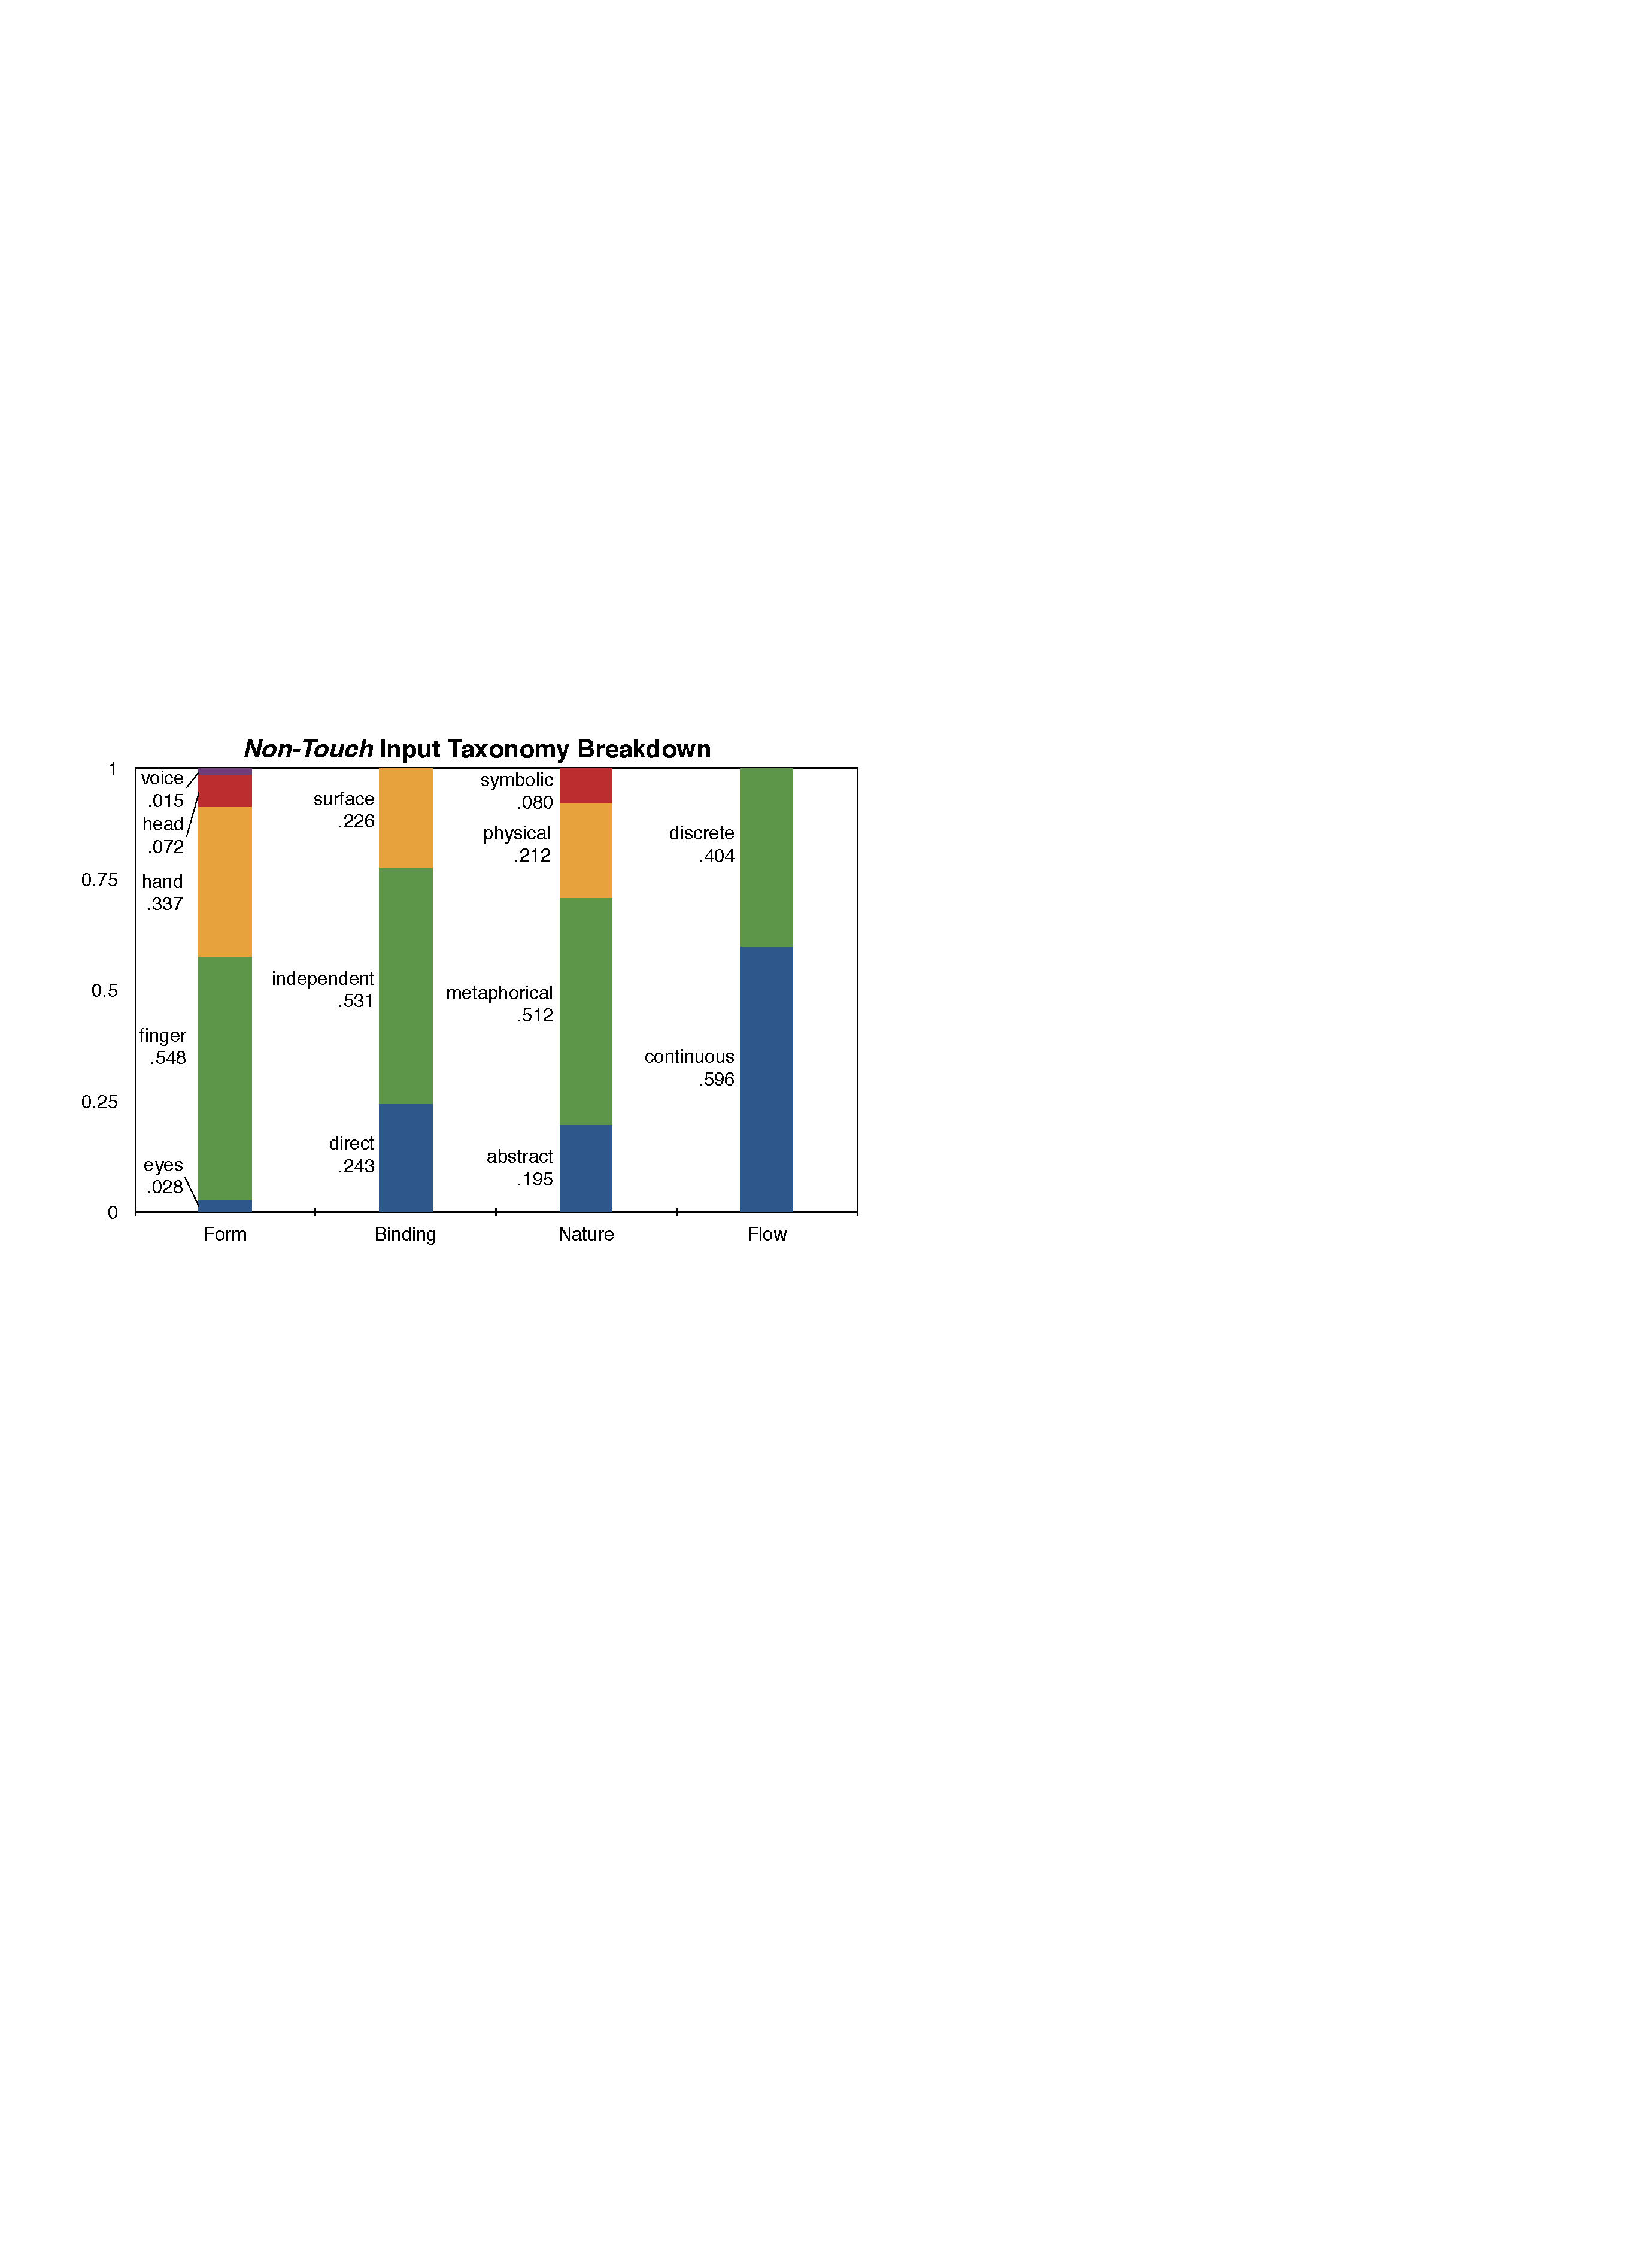
\includegraphics[width=1\columnwidth]{Figures/InAirTaxonomy}
  \caption{Percentage of game inputs in each taxonomy dimension with \emph{non-touch} interaction.}
  \label{fig:InAirTaxonomy}
  \end{figure} 

  \section{User-Defined Game Input Set}
  The goal of this work is to present a user-defined game input set for smart glasses used in a public environment. This section gives the process by which the set was created and properties of the set. Unlike the input sets for existing games on smart glasses, the set we have found is based on observed user behavior.

   \subsection{Agreement}
	All 24 participants have provided game input for each and every game task, smart glasses form and interaction method. For each game task, we made groups of identical actions used by participants. Group size was then used to compute an \emph{Agreement Score} that reflects the consensus among participants regarding the action used for a certain game task. A task with a .31 agreement score means that, two randomly picked participants will have a 31\% chance to perform an identical input action for this task. The definition and formula of the agreement score can be found in previous work. \cite{Wobbrock:2005:MGS:1056808.1057043}.
   \begin{equation}
   A = \frac{\displaystyle{\sum_{t\epsilon T }} \sum_{P_i \subseteq P_t } \left(\frac{\lvert{P_i}\rvert}{\lvert{P_t}\rvert}\right) ^ 2}{\displaystyle{\lvert{T}\rvert}}
   \end{equation}
  
   In eq. 1, $t$ is a task in the set of all tasks $T$, $P_{t}$ is the set of proposed input actions for task $t$, and $P_i$ is a subset of identical input actions from $P_{t}$. The range for $A$ is $\left[\lvert{P_t}\rvert ^{-1}, 1\right]$. As an example, consider the agreement for \emph{draw a path} with \emph{touch} input, it had four groups of identical input actions with group sizes 34, 4, 5 and 5. we compute

   \begin{equation}
   A_{touch-path} = \left(\frac{34}{48}\right) ^ 2  + \left(\frac{4}{48}\right) ^ 2 + \left(\frac{5}{48}\right) ^ 2 + \left(\frac{5}{48}\right) ^ 2 = 0.53
   \end{equation}

The participant agreement for our study is pictured in Figure \ref{fig:Agreement}. The overall agreement for \emph{touch} and \emph{non-touch} inputs were $A_{touch}$=0.25 and $A_{non-touch}$=0.27, respectively. When comparing the agreement of \emph{touch} and \emph{non-touch} inputs, we clearly see that their patterns are extremely similar. The average difference of agreement between these two interaction methods was .056. This implies that the agreement score was influenced more by the game tasks than by the interaction methods.


 \begin{figure}[!h]
  \centering
  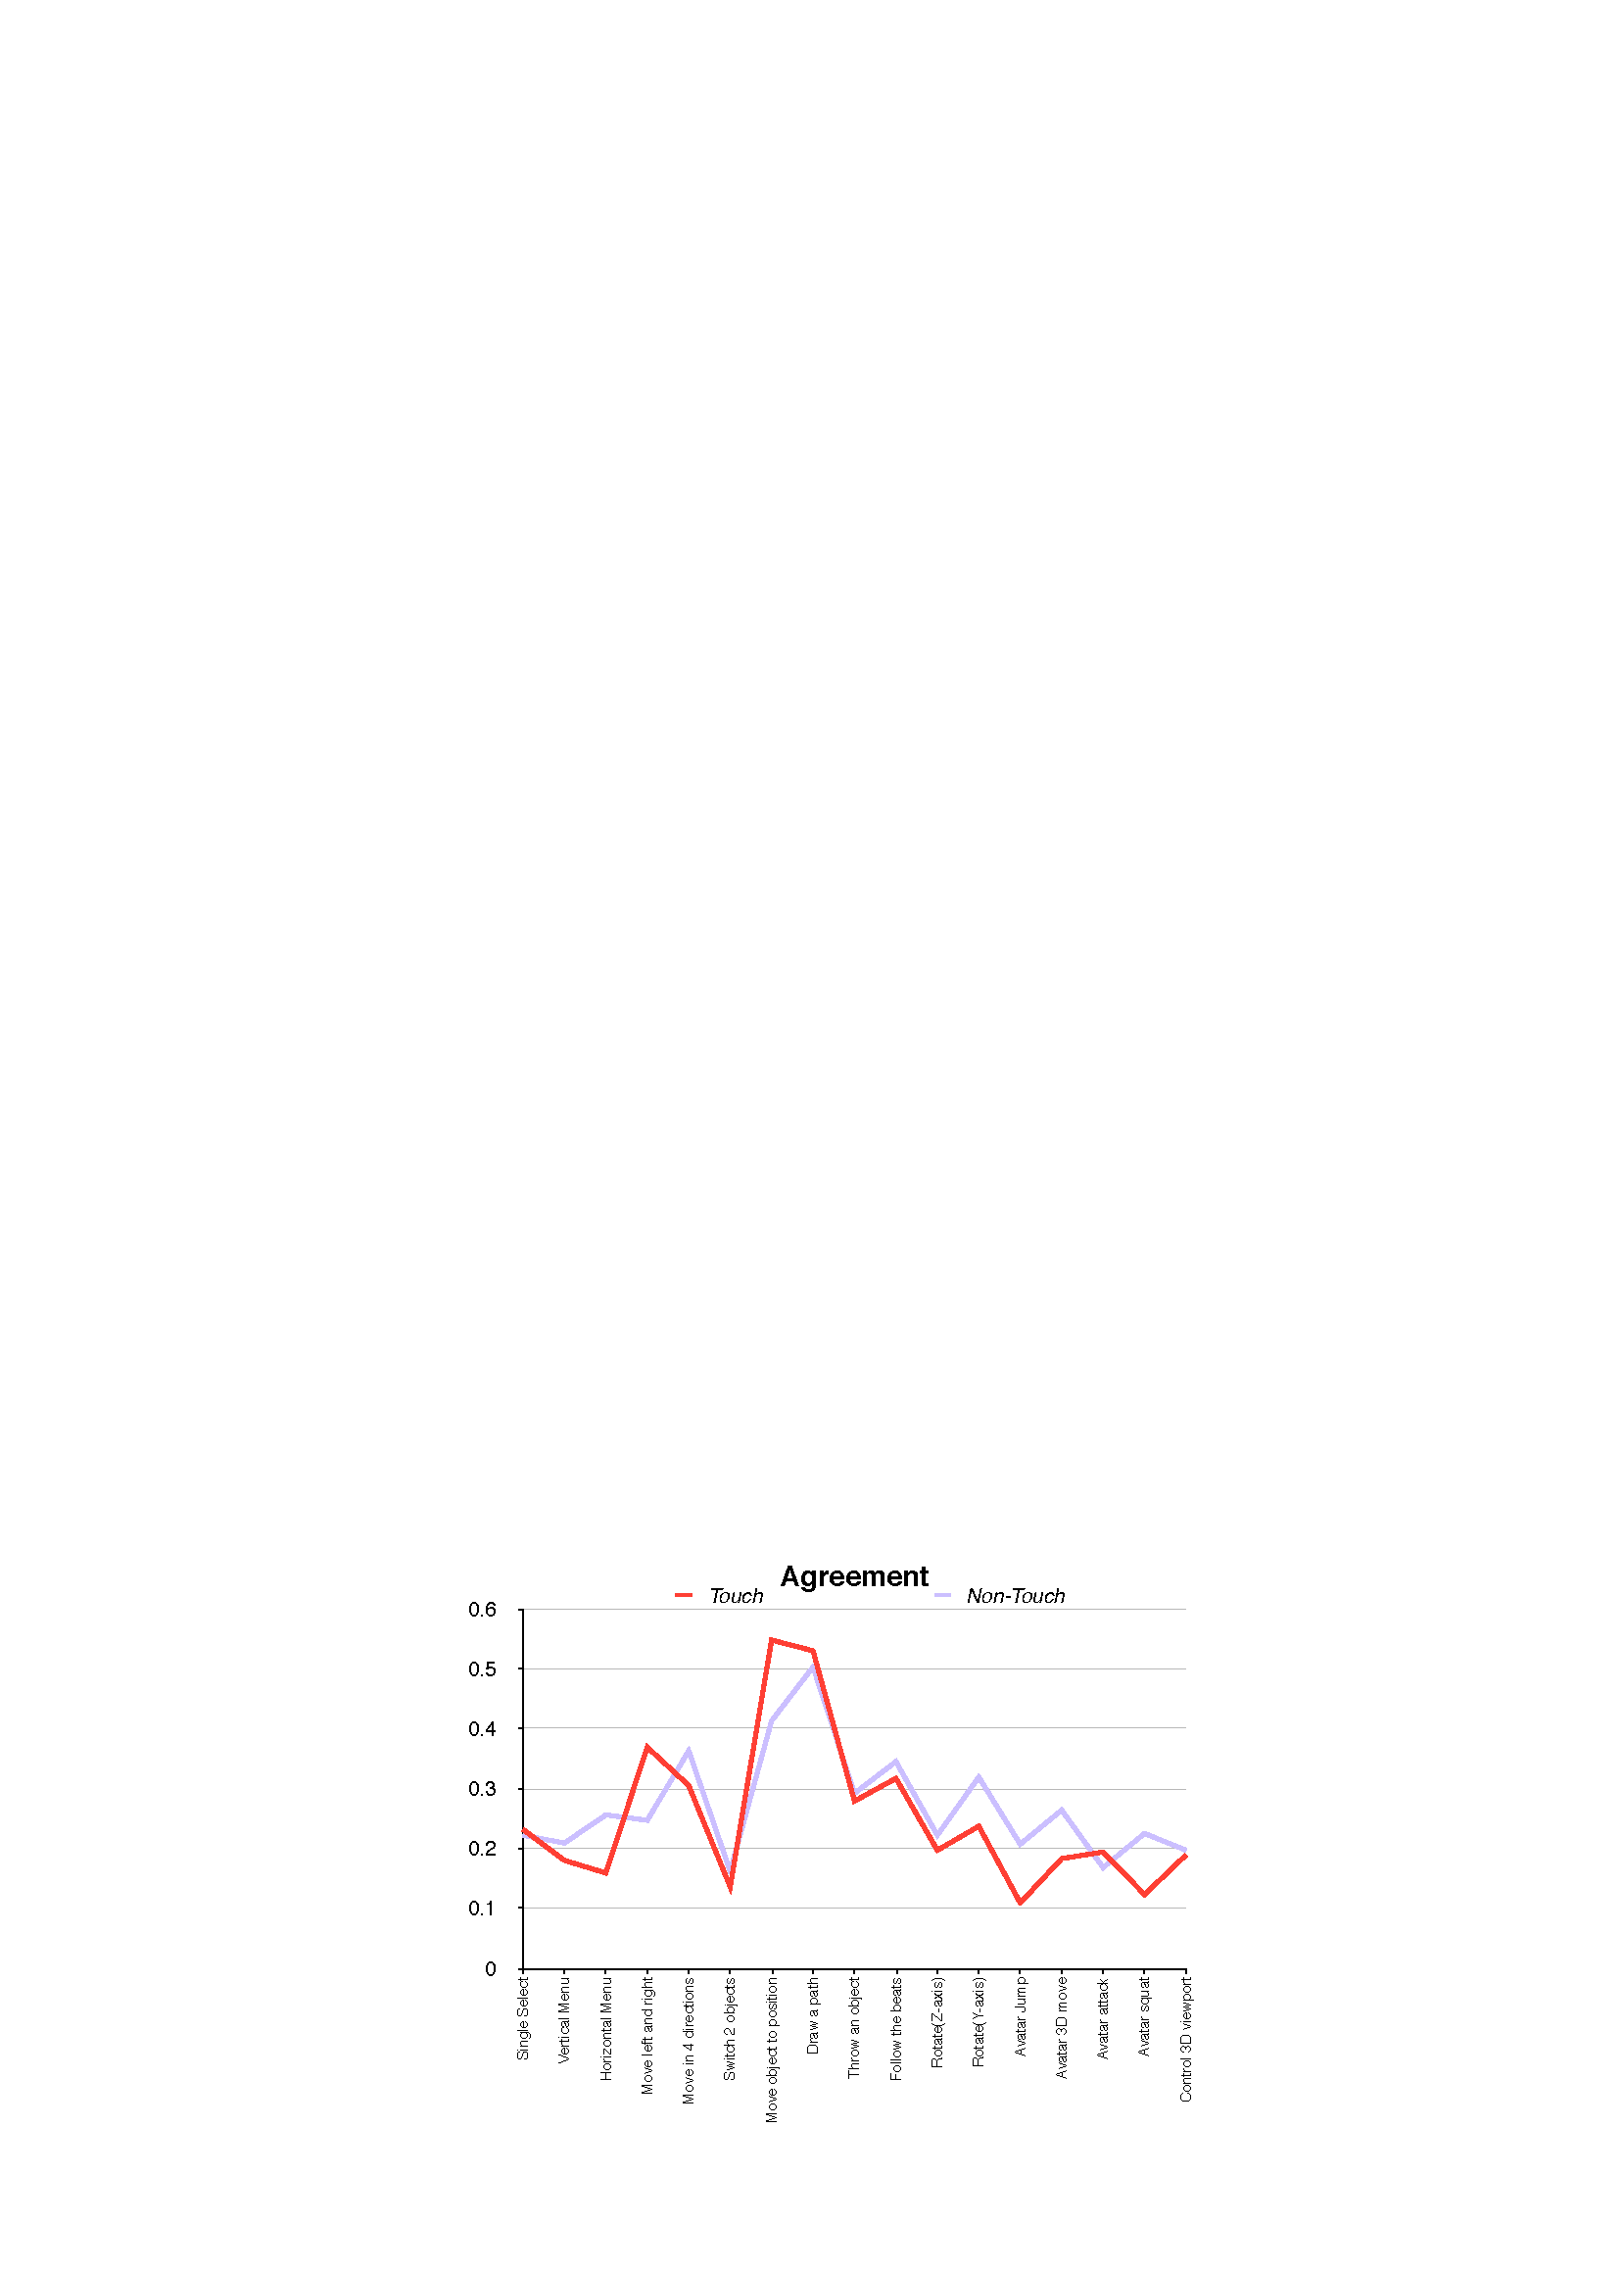
\includegraphics[width=1\columnwidth]{Figures/Agreement}

  \caption{Agreement for each game task. The tasks are listed in the same order as they appear in Table \ref{tab:table1}.}
  \label{fig:Agreement}
  \end{figure} 

   %\subsubsection{Conflict and Coverage}

   %Howerver, where the same control action was used to perform different game tasks, a conflict occurred if the game consists the tasks at same time. In our case ,we found that ``Move in 4 Directions'',``Avatar 3D Move'' and ``Viewport Controls'' are assigned with same control action with on-body input(Fig?.?). According to the property of our top 90 casual games, the average task count for these game is 2.56 (std=1.07). In another word, there are about 1 to 4 game tasks in each game title. There is a low chance to perform these three game controls at same game and same time. To make our game control set reflects more consistent with user behavior, we decide to remain it conflict. 

 \begin{figure}
  \centering
  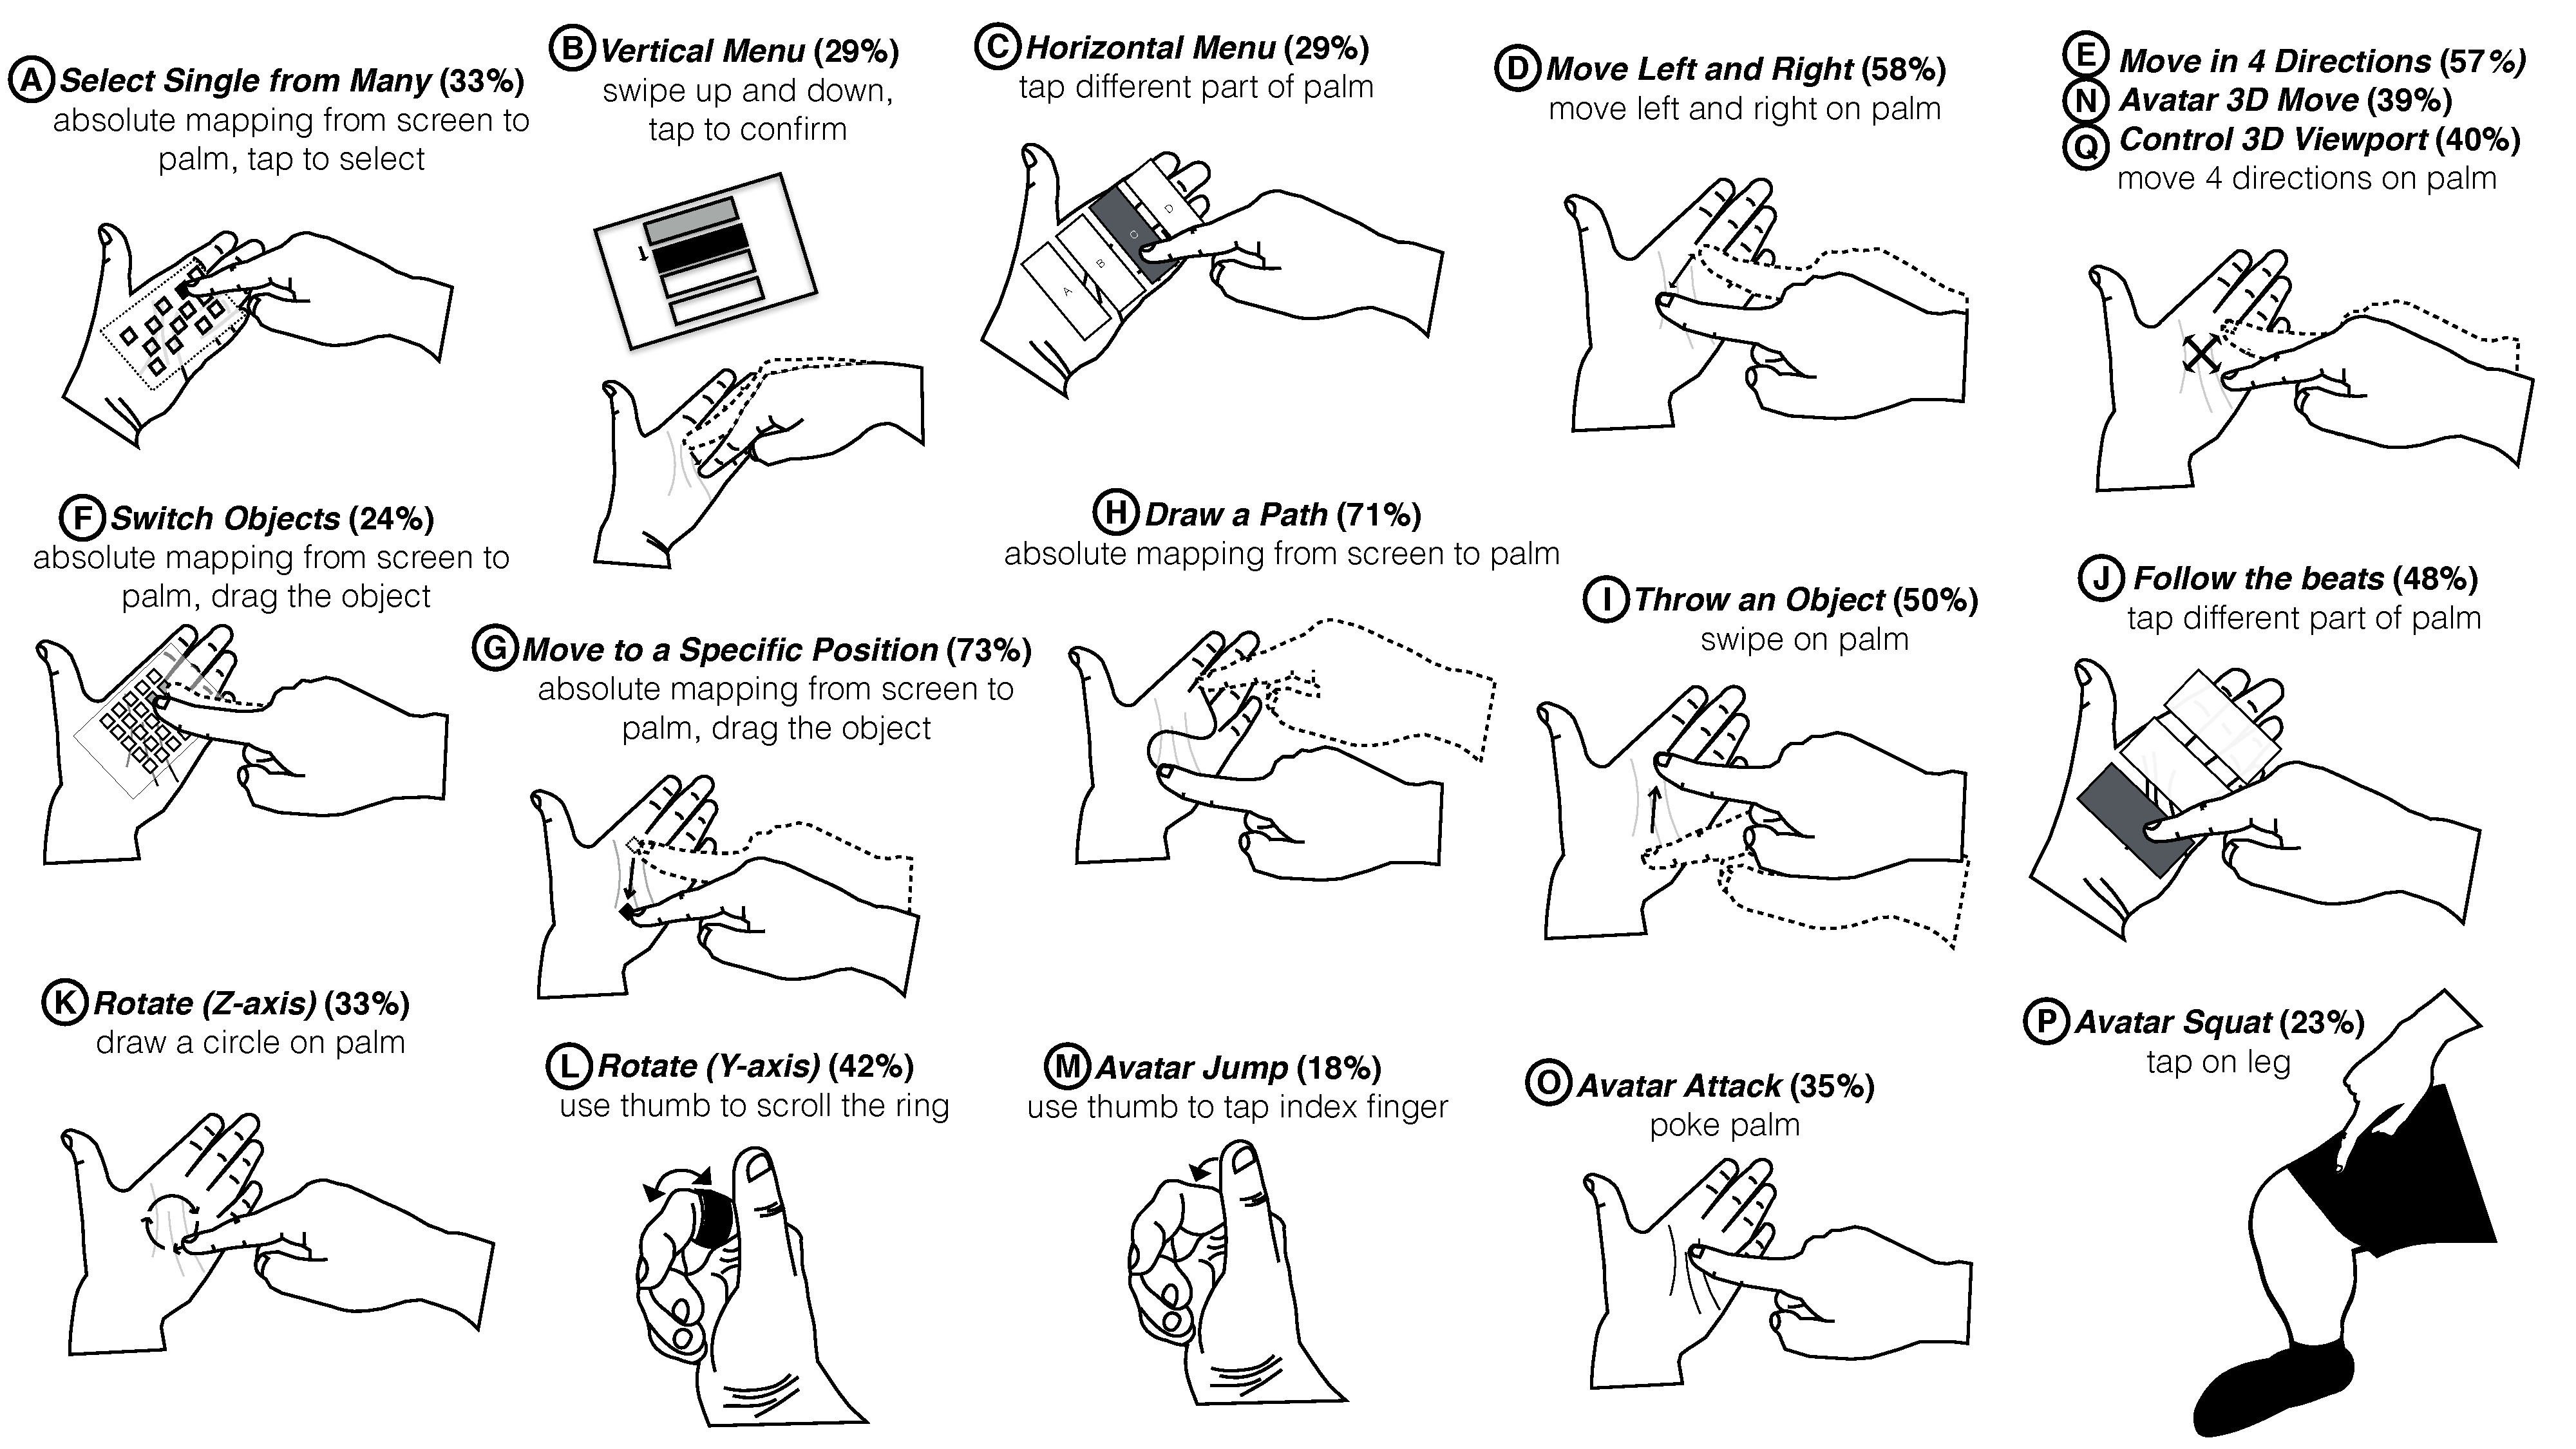
\includegraphics[width=1\textwidth]{Figures/OnBodyInputSet}
  \caption{The user-defined game input set with \emph{touch} inputs. The percentages indicate the portion of users who performed the pictured input action for the game task. Note that, there are 3 tasks (``Move in 4 directions'', ``Avatar 3D Move'', and ``Control 3D viewport'') have been assigned with an identical input action.}
  \label{fig:OnBodyInputSet}
  \end{figure}

  \begin{figure}
  \centering
  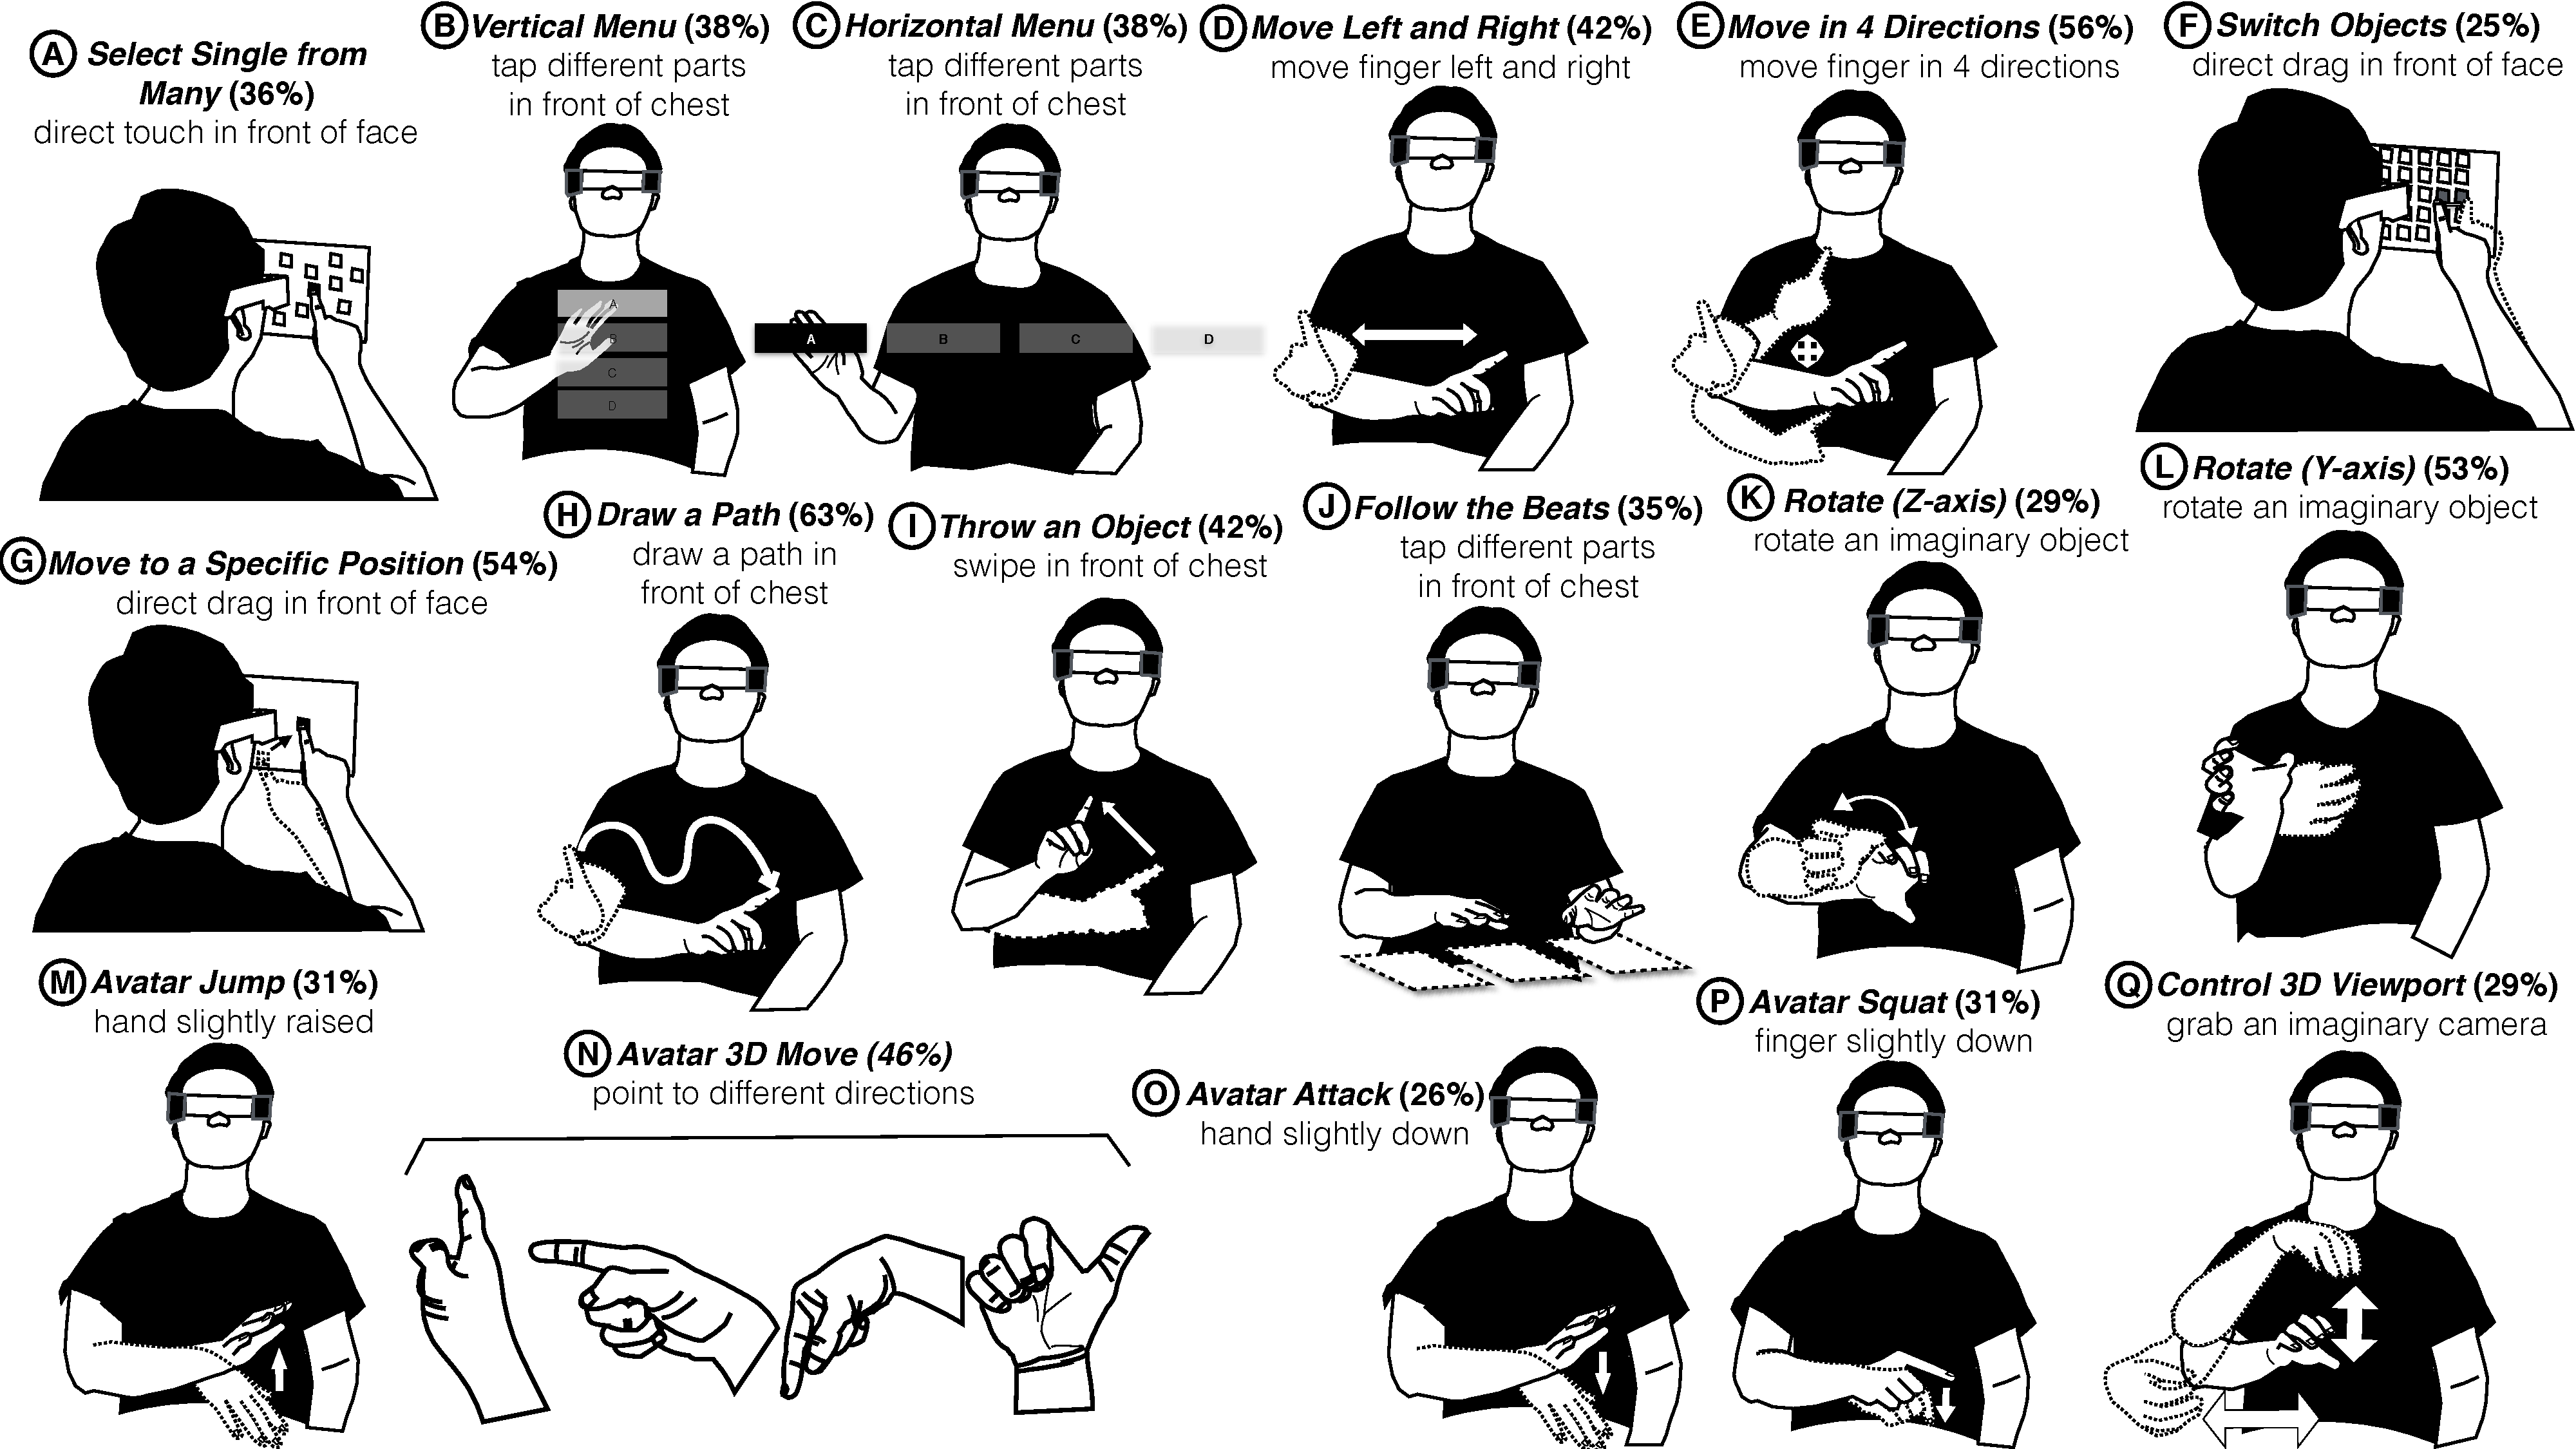
\includegraphics[width=1\textwidth]{Figures/InAirSet}
  \caption{The user-defined game input set with \emph{non-touch} interaction, The percentages indicate the portion of users who performed the pictured input action for the game task.}
  \label{fig:InAirSet}
  \end{figure}


   \subsection{Properties of the User-defined Game Input Set}
   The user-defined game input set was developed by taking the largest groups with identical input actions for each game task and assigning those actions to the game tasks. 
   The resulting user-defined game input set covers 41.32\% and 40.07\% of all game inputs proposed for both the \emph{touch} and the \emph{non-touch} interaction class respectively.
   Our user defined set is useful, therefore, not just for what it contains, but also for what it omits.

      All the inputs in our final \emph{touch} input set are finger based (see Figure \ref{fig:OnBodyInputSet}). Most of them use a single finger tip to perform gestures on different surfaces. The most preferable surface for \emph{touch} input is the hand palm. This way, the hand palm acts as a trackpad or a proxy touch-screen. The other touch inputs are finger interactions with single hand. More specifically, participants used their thumb to interact with their index finger or the ring on the finger.

   For \emph{non-touch} input set (see Figure \ref{fig:InAirSet}), even though we informed users beforehand that they were not limited to using their hands when providing game input, the results show that users still preferred to use hand input over voice control, eye gestures and head tilting. Additionally, users would make use of direct-control if they had to perform precise tasks, such as selecting an object from many or moving an object to a specific position. On the other hand, for tasks with lower precision requirements, such as selecting a single option from 4 or making an avatar jump, users would prefer using an indirect-control. For examples: the user taps 4 different areas in front of their chest or the user raises his hands slightly.


 

   \subsection{Taxonometric Breakdown of User-Defined Game Inputs}
   As expected, the taxonometric breakdown of the final user-defined game input set (Figure \ref{fig:OnBodyInputSet} and \ref{fig:InAirSet}) is similar to the proportions of all control actions proposed (Figure \ref{fig:OnBodyTaxonomy} and \ref{fig:InAirTaxonomy}). Across all taxonomy categories, the average difference between these two sets was only 5.61\%, (\emph{touch} input 6.31\% and \emph{non-touch} input 4.91\%, respectively).

  \section{Mental Model Observations}
    \subsection{Social Acceptance and Input Area}
    To our surprise, approximately 63\% of the in-air gestures were not performed in front of the face (See Figure \ref{fig:figureInAirPorpotion}.2). This behavior conflicts with the current ``Google Glass'' design. There were 7 participants who performed most gestures in front of their face. They indicated that input in front of the face was more precise and intuitive. At the same time, the other 17 participants preferred to perform in-air gestures in front of or below their chest. Among them, there were 3 participants who didn't perform a single in-air gesture in front of their face. These users indicated that moving a finger in front of their face was weird and not socially acceptable. They also noted that there was a hand fatigue problem if they had to lift their hand in front of their face all the time, so they thought that it was not suitable for gaming.

    \subsection{Bias by Existing Game Input}
    Although we were careful not to show elements from traditional game platforms like PCs, consoles and mobile games, participants still often reasoned based on their previous gaming experience. For example, some input actions were performed as if using a touch-screen in front of their face (see Figure \ref{fig:InAirSet}\{A,F,G\}). Some actions were like using an imaginary trackpad on an in-air surface or on the hand palm(see Figure \ref{fig:OnBodyInputSet}\{B,D,E,H,I,K,N,Q\} and Figure \ref{fig:InAirSet}\{H,I\}). Even with simple shapes and basic characters, it was clear how deeply rooted the previous gaming experience is. Some quotes reveal this: ``So I just click a button like on a game controller'', ``Can I just imagine there is a trackpad on my palm?'' and ``It's an imaginary touch-screen.''
 

\subsection{Identical Gestures on Different Surfaces}
 In our study, we found several identical gestures performed by our users on different surfaces. Take the task ``Move in 4 directions'' for example, although 57\% of the gestures were performed by moving a finger on the palm with \emph{touch} inputs(Figure \ref{fig:OnBodyInputSet}.E). The rest of the gestures were mostly using identical gestures (moving a finger), but then on the different surfaces such as the back of the hand, the leg, the forearm and on the even face. The same phenomenon could also be observed when comparing the game input of the user-defined input set with \emph{touch} and \emph{non-touch} inputs for the tasks ``Move left and right'', ``Move in 4 directions'', ``Draw a Path'', ``Throw an Object''. Participants used the hand palm or an imaginary in-air surface. 
 (See Figure \ref{fig:OnBodyInputSet} and Figure \ref{fig:InAirSet} \{D,E,H,I\}). 

 In these cases, the surface did not influence the meaning of the gestures. We have asked users why they chose the palm as their input area. The general response was that it required the least physical movement, such as ``I chose the left palm to perform a gesture on because it is near to my right hand''. 


  \begin{figure}[!b]
  \centering
  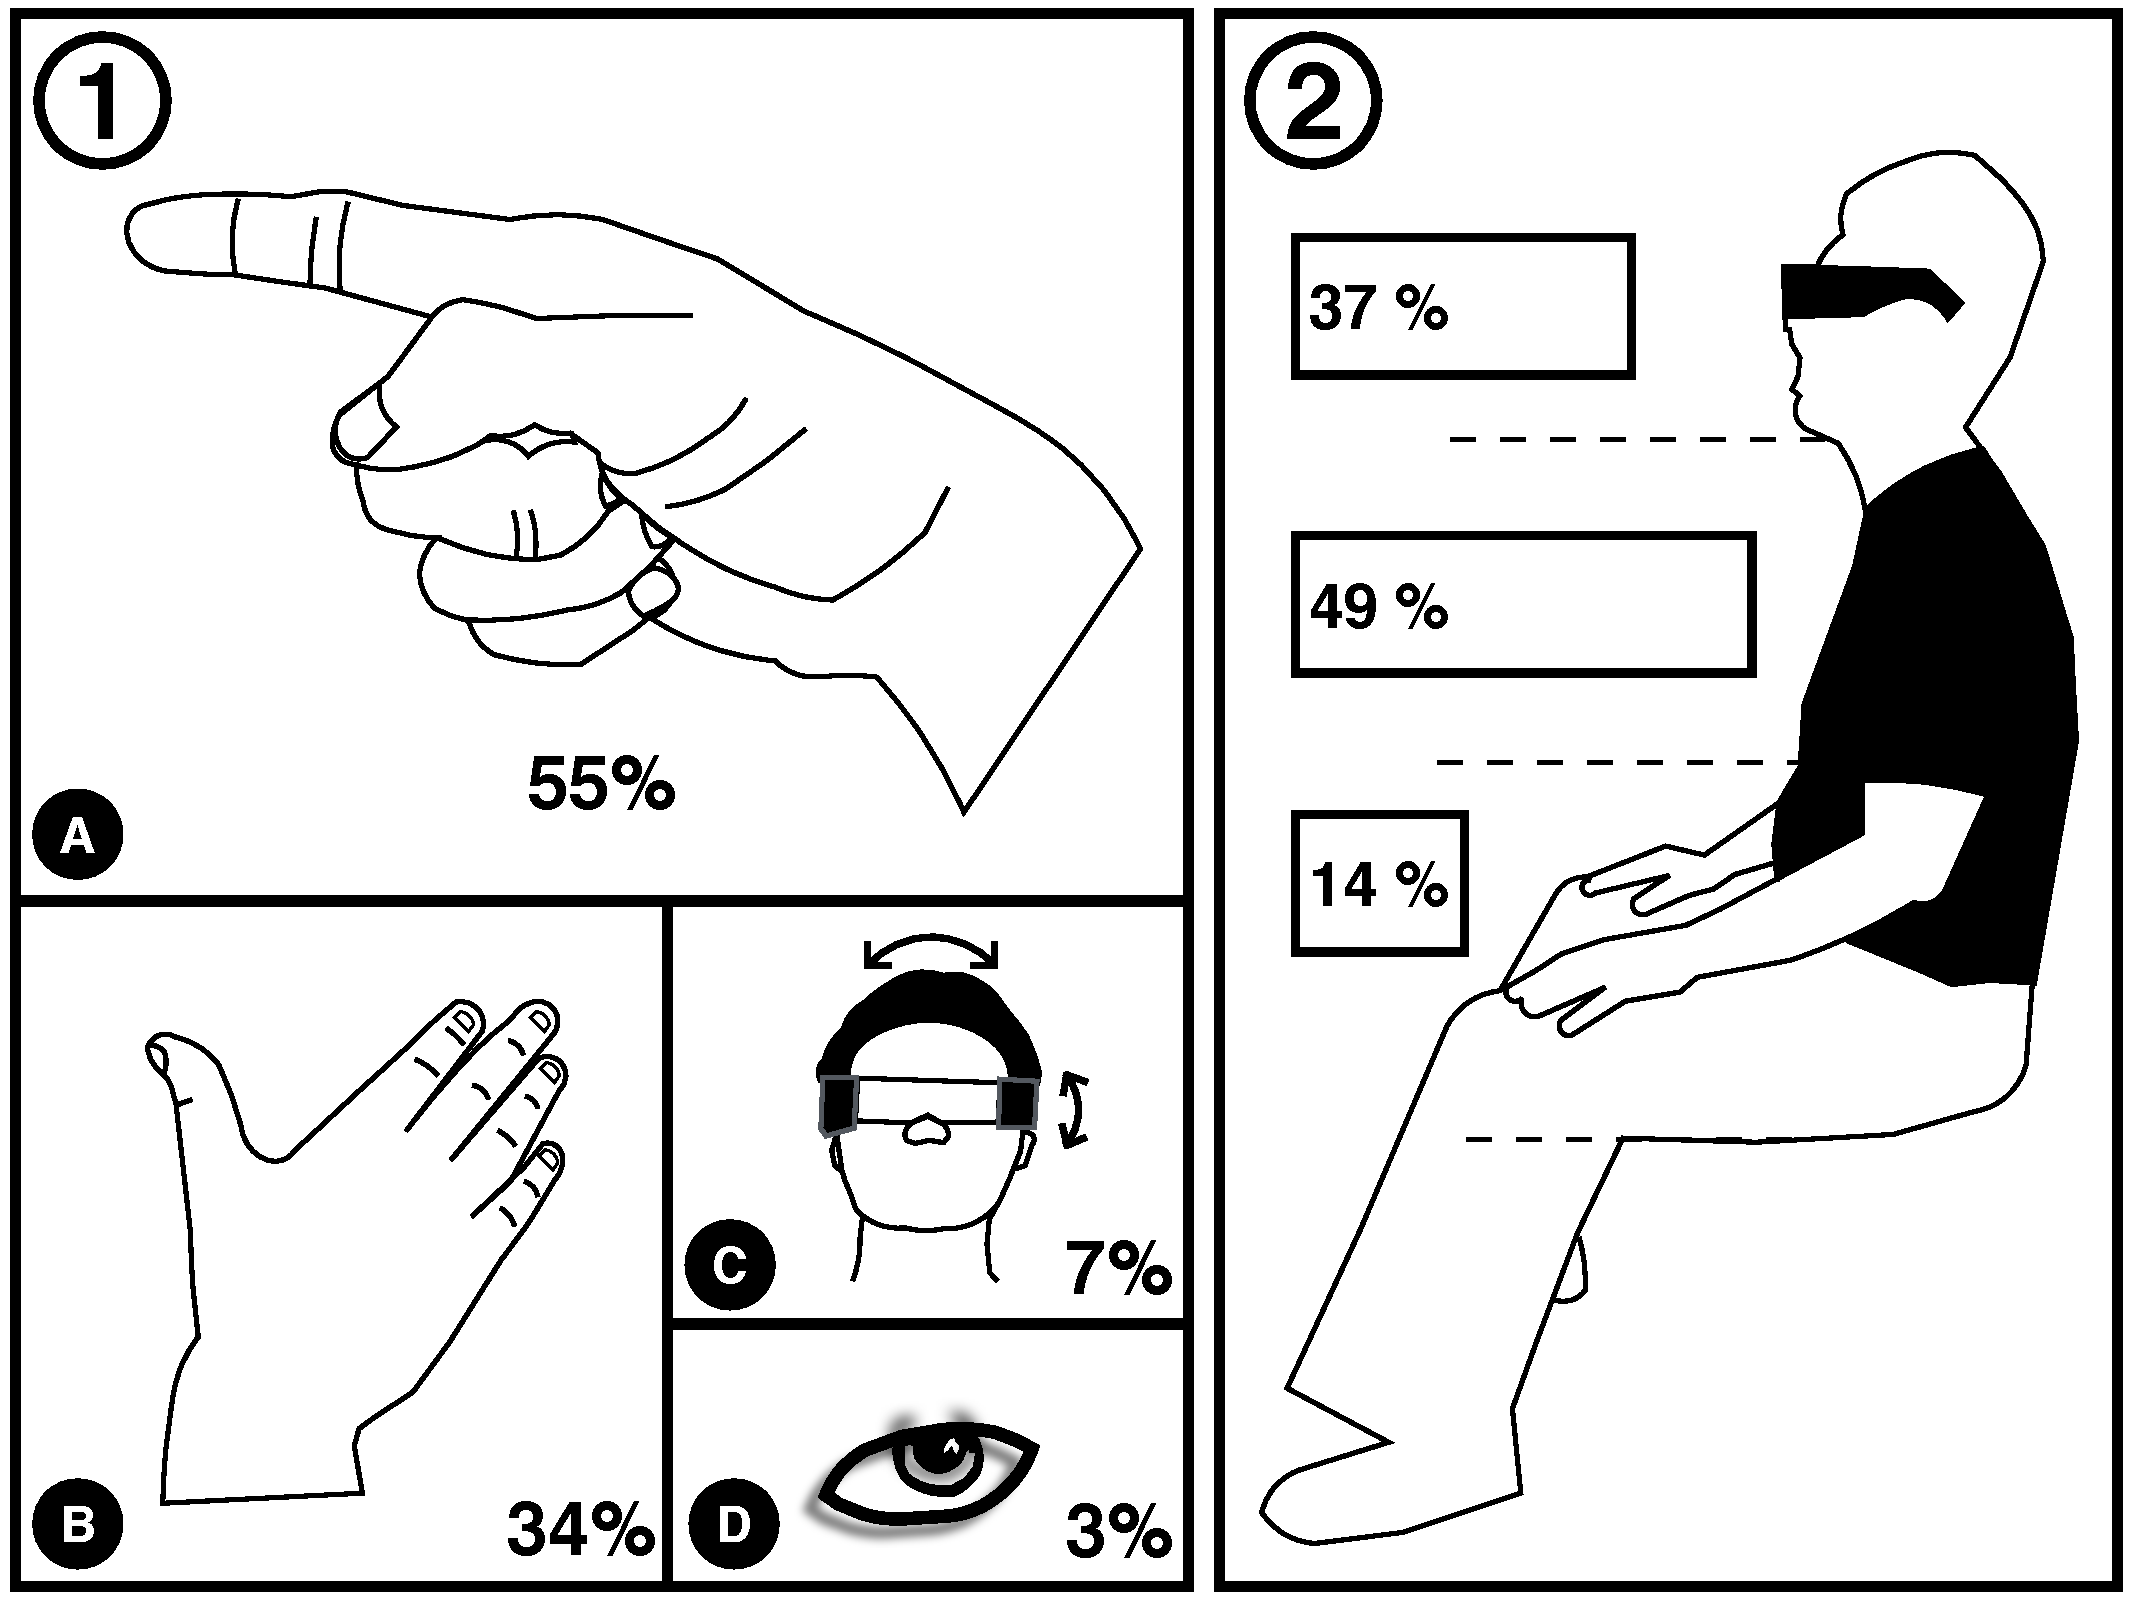
\includegraphics[width=0.8\columnwidth]{Figures/InAirControlArea}
  \caption{1.The top 4 \emph{non-touch} interaction forms. Percentages indicate the portion of \emph{non-touch} game inputs that consisted of the pictured input. (A)Using a finger to perform an in-air gesture. (B)Using the full hand to perform an in-air gesture. (C)Using head-tilting to perform game input. (D)Using eye-gestures to perform game input. 2.The distribution of the in-air gesture input area. Half of the in-air gestures (49\%) were performed in front of the chest, 14\% in front of or below the belly, and only 37\% of the gestures were performed in front of the face.}
  \label{fig:figureInAirPorpotion}
  \end{figure}

\begin{figure}
    \centering
    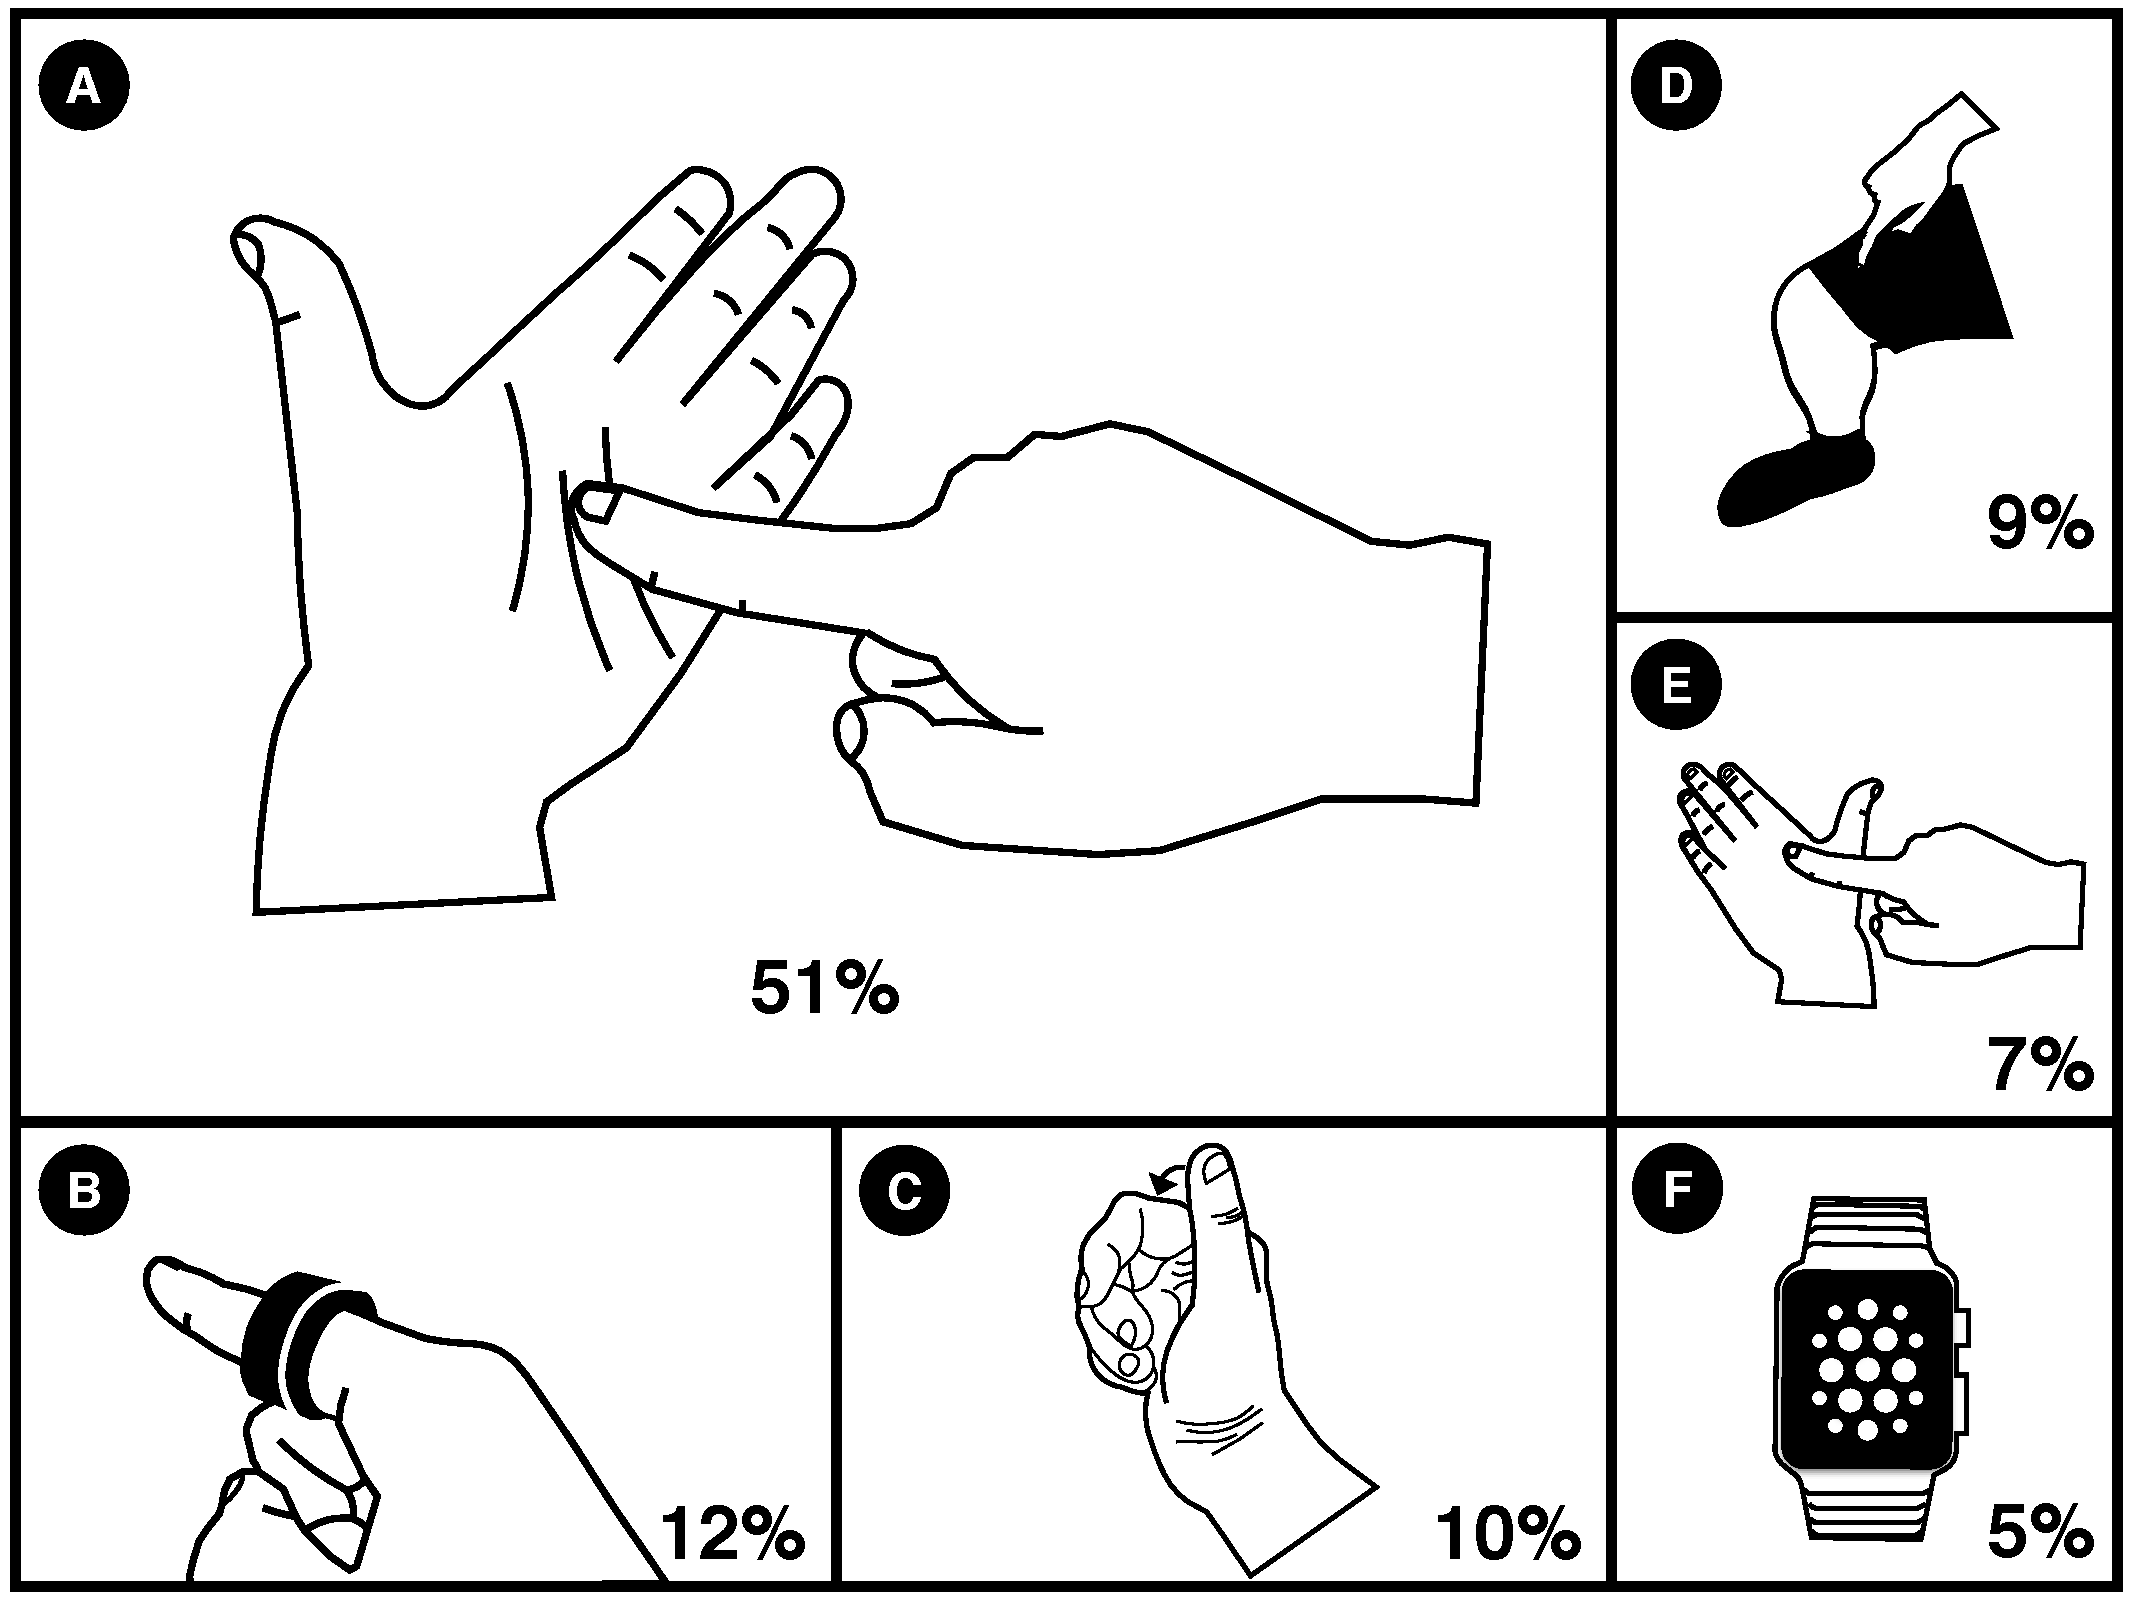
\includegraphics[width=0.8\columnwidth]{Figures/OnBodyForms}
    \caption{The top 6 \emph{touch} input forms. Percentage indicates the portion of \emph{touch} input actions. (A)Interaction between finger and palm. (B)Interaction between finger and ring. (C)Interaction between fingers. (D)Interaction between finger and leg. (E)Interaction between finger and back of hand. (F)Interaction between finger and watch.}
    \label{fig:figureOnBodyPorpotion}
    \end{figure}  